\documentclass[convert={density=300,outext=.png}]{standalone}
\usepackage{tikz}
\begin{document}
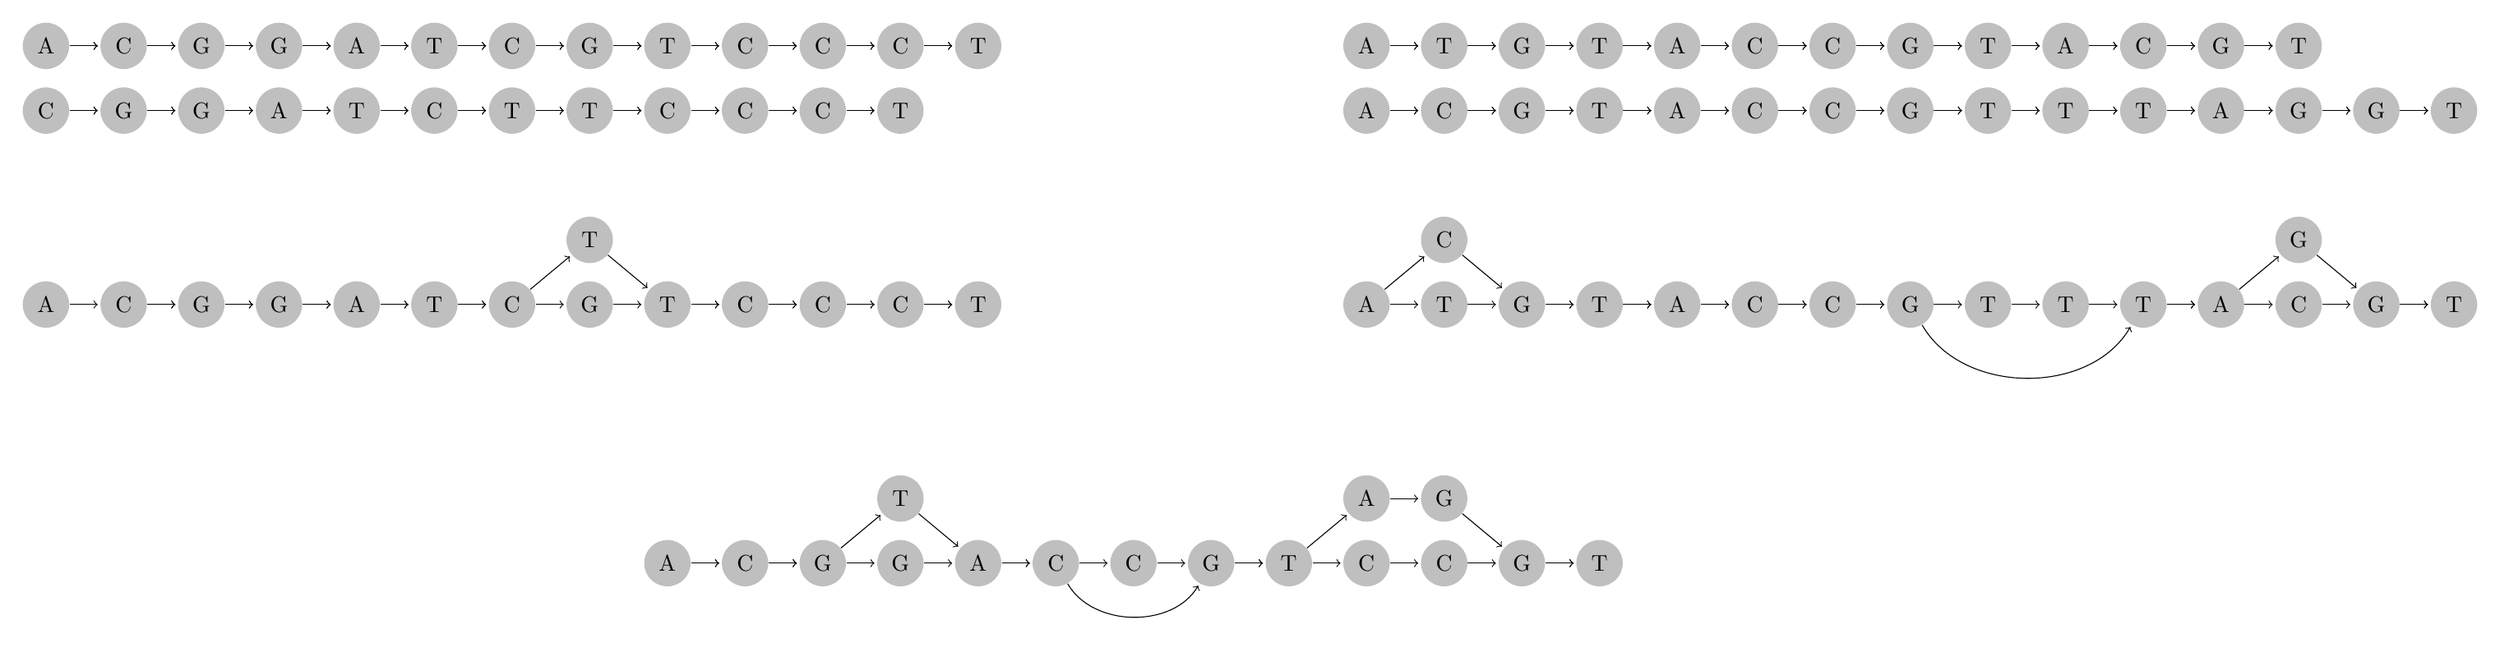
\begin{tikzpicture}[shorten >=1pt,->]
  \def\f{1.2};
  \def\fy{1}

\tikzstyle{vertex}=[circle,fill=black!25,minimum size=17*\f pt,inner sep=0pt]
ACGGAC-GTCCGT
\node[vertex][] (P1) at (0*\f,0) {A};
\node[vertex][] (P2) at (1*\f,0) {C};
\draw (P1) -- (P2);
\draw (P1) -- (P2);
\node[vertex][] (P3) at (2*\f,0) {G};
\draw (P2) -- (P3);
\draw (P2) -- (P3);
\node[vertex][] (P4) at (3*\f,0) {G};
\draw (P3) -- (P4);
\draw (P3) -- (P4);
\node[vertex][] (P5) at (4*\f,0) {A};
\draw (P4) -- (P5);
\draw (P4) -- (P5);
\node[vertex][] (P6) at (5*\f,0) {T};
\draw (P5) -- (P6);
\draw (P5) -- (P6);
\node[vertex][] (P7) at (6*\f,0) {C};
\draw (P6) -- (P7);
\draw (P6) -- (P7);
\node[vertex][] (P8) at (7*\f,0) {G};
\draw (P7) -- (P8);
\draw (P7) -- (P8);
\node[vertex][] (P9) at (8*\f,0) {T};
\draw (P8) -- (P9);
\draw (P8) -- (P9);
\node[vertex][] (P10) at (9*\f,0) {C};
\draw (P9) -- (P10);
\draw (P9) -- (P10);
\node[vertex][] (P11) at (10*\f,0) {C};
\draw (P10) -- (P11);
\draw (P10) -- (P11);
\node[vertex][] (P12) at (11*\f,0) {C};
\draw (P11) -- (P12);
\draw (P11) -- (P12);
\node[vertex][] (P13) at (12*\f,0) {T};
\draw (P12) -- (P13);
\draw (P12) -- (P13);
\node[vertex][] (P14) at (0*\f,-1) {C};
\node[vertex][] (P15) at (1*\f,-1) {G};
\draw (P14) -- (P15);
\draw (P14) -- (P15);
\node[vertex][] (P16) at (2*\f,-1) {G};
\draw (P15) -- (P16);
\draw (P15) -- (P16);
\node[vertex][] (P17) at (3*\f,-1) {A};
\draw (P16) -- (P17);
\draw (P16) -- (P17);
\node[vertex][] (P18) at (4*\f,-1) {T};
\draw (P17) -- (P18);
\draw (P17) -- (P18);
\node[vertex][] (P19) at (5*\f,-1) {C};
\draw (P18) -- (P19);
\draw (P18) -- (P19);
\node[vertex][] (P20) at (6*\f,-1) {T};
\draw (P19) -- (P20);
\draw (P19) -- (P20);
\node[vertex][] (P21) at (7*\f,-1) {T};
\draw (P20) -- (P21);
\draw (P20) -- (P21);
\node[vertex][] (P22) at (8*\f,-1) {C};
\draw (P21) -- (P22);
\draw (P21) -- (P22);
\node[vertex][] (P23) at (9*\f,-1) {C};
\draw (P22) -- (P23);
\draw (P22) -- (P23);
\node[vertex][] (P24) at (10*\f,-1) {C};
\draw (P23) -- (P24);
\draw (P23) -- (P24);
\node[vertex][] (P25) at (11*\f,-1) {T};
\draw (P24) -- (P25);
\draw (P24) -- (P25);
\node[vertex][] (P26) at (17*\f,0) {A};
\node[vertex][] (P27) at (18*\f,0) {T};
\draw (P26) -- (P27);
\draw (P26) -- (P27);
\node[vertex][] (P28) at (19*\f,0) {G};
\draw (P27) -- (P28);
\draw (P27) -- (P28);
\node[vertex][] (P29) at (20*\f,0) {T};
\draw (P28) -- (P29);
\draw (P28) -- (P29);
\node[vertex][] (P30) at (21*\f,0) {A};
\draw (P29) -- (P30);
\draw (P29) -- (P30);
\node[vertex][] (P31) at (22*\f,0) {C};
\draw (P30) -- (P31);
\draw (P30) -- (P31);
\node[vertex][] (P32) at (23*\f,0) {C};
\draw (P31) -- (P32);
\draw (P31) -- (P32);
\node[vertex][] (P33) at (24*\f,0) {G};
\draw (P32) -- (P33);
\draw (P32) -- (P33);
\node[vertex][] (P34) at (25*\f,0) {T};
\draw (P33) -- (P34);
\draw (P33) -- (P34);
\node[vertex][] (P35) at (26*\f,0) {A};
\draw (P34) -- (P35);
\draw (P34) -- (P35);
\node[vertex][] (P36) at (27*\f,0) {C};
\draw (P35) -- (P36);
\draw (P35) -- (P36);
\node[vertex][] (P37) at (28*\f,0) {G};
\draw (P36) -- (P37);
\draw (P36) -- (P37);
\node[vertex][] (P38) at (29*\f,0) {T};
\draw (P37) -- (P38);
\draw (P37) -- (P38);
\node[vertex][] (P39) at (17*\f,-1) {A};
\node[vertex][] (P40) at (18*\f,-1) {C};
\draw (P39) -- (P40);
\draw (P39) -- (P40);
\node[vertex][] (P41) at (19*\f,-1) {G};
\draw (P40) -- (P41);
\draw (P40) -- (P41);
\node[vertex][] (P42) at (20*\f,-1) {T};
\draw (P41) -- (P42);
\draw (P41) -- (P42);
\node[vertex][] (P43) at (21*\f,-1) {A};
\draw (P42) -- (P43);
\draw (P42) -- (P43);
\node[vertex][] (P44) at (22*\f,-1) {C};
\draw (P43) -- (P44);
\draw (P43) -- (P44);
\node[vertex][] (P45) at (23*\f,-1) {C};
\draw (P44) -- (P45);
\draw (P44) -- (P45);
\node[vertex][] (P46) at (24*\f,-1) {G};
\draw (P45) -- (P46);
\draw (P45) -- (P46);
\node[vertex][] (P47) at (25*\f,-1) {T};
\draw (P46) -- (P47);
\draw (P46) -- (P47);
\node[vertex][] (P48) at (26*\f,-1) {T};
\draw (P47) -- (P48);
\draw (P47) -- (P48);
\node[vertex][] (P49) at (27*\f,-1) {T};
\draw (P48) -- (P49);
\draw (P48) -- (P49);
\node[vertex][] (P50) at (28*\f,-1) {A};
\draw (P49) -- (P50);
\draw (P49) -- (P50);
\node[vertex][] (P51) at (29*\f,-1) {G};
\draw (P50) -- (P51);
\draw (P50) -- (P51);
\node[vertex][] (P52) at (30*\f,-1) {G};
\draw (P51) -- (P52);
\draw (P51) -- (P52);
\node[vertex][] (P53) at (31*\f,-1) {T};
\draw (P52) -- (P53);
\draw (P52) -- (P53);
\node[vertex][] (P54) at (0*\f,-4) {A};
\node[vertex][] (P55) at (1*\f,-4) {C};
\draw (P54) -- (P55);
\node[vertex][] (P56) at (2*\f,-4) {G};
\draw (P55) -- (P56);
\draw (P55) -- (P56);
\node[vertex][] (P57) at (3*\f,-4) {G};
\draw (P56) -- (P57);
\draw (P56) -- (P57);
\node[vertex][] (P58) at (4*\f,-4) {A};
\draw (P57) -- (P58);
\draw (P57) -- (P58);
\node[vertex][] (P59) at (5*\f,-4) {T};
\draw (P58) -- (P59);
\draw (P58) -- (P59);
\node[vertex][] (P60) at (6*\f,-4) {C};
\draw (P59) -- (P60);
\draw (P59) -- (P60);
\node[vertex][] (P61) at (7*\f,-4) {G};
\draw (P60) -- (P61);
\node[vertex][] (P62) at (7*\f,-3) {T};
\draw (P60) -- (P62);
\node[vertex][] (P63) at (8*\f,-4) {T};
\draw (P61) -- (P63);
\draw (P62) -- (P63);
\node[vertex][] (P64) at (9*\f,-4) {C};
\draw (P63) -- (P64);
\draw (P63) -- (P64);
\node[vertex][] (P65) at (10*\f,-4) {C};
\draw (P64) -- (P65);
\draw (P64) -- (P65);
\node[vertex][] (P66) at (11*\f,-4) {C};
\draw (P65) -- (P66);
\draw (P65) -- (P66);
\node[vertex][] (P67) at (12*\f,-4) {T};
\draw (P66) -- (P67);
\draw (P66) -- (P67);
\node[vertex][] (P68) at (17*\f,-4) {A};
\node[vertex][] (P69) at (18*\f,-4) {T};
\draw (P68) -- (P69);
\node[vertex][] (P70) at (18*\f,-3) {C};
\draw (P68) -- (P70);
\node[vertex][] (P71) at (19*\f,-4) {G};
\draw (P69) -- (P71);
\draw (P70) -- (P71);
\node[vertex][] (P72) at (20*\f,-4) {T};
\draw (P71) -- (P72);
\draw (P71) -- (P72);
\node[vertex][] (P73) at (21*\f,-4) {A};
\draw (P72) -- (P73);
\draw (P72) -- (P73);
\node[vertex][] (P74) at (22*\f,-4) {C};
\draw (P73) -- (P74);
\draw (P73) -- (P74);
\node[vertex][] (P75) at (23*\f,-4) {C};
\draw (P74) -- (P75);
\draw (P74) -- (P75);
\node[vertex][] (P76) at (24*\f,-4) {G};
\draw (P75) -- (P76);
\draw (P75) -- (P76);
\node[vertex][] (P77) at (25*\f,-4) {T};
\draw (P76) -- (P77);
\node[vertex][] (P78) at (26*\f,-4) {T};
\draw (P77) -- (P78);
\node[vertex][] (P79) at (27*\f,-4) {T};
\path [->] (P76) edge[bend right=60] node {} (P79);
\draw (P78) -- (P79);
\node[vertex][] (P80) at (28*\f,-4) {A};
\draw (P79) -- (P80);
\draw (P79) -- (P80);
\node[vertex][] (P81) at (29*\f,-4) {C};
\draw (P80) -- (P81);
\node[vertex][] (P82) at (29*\f,-3) {G};
\draw (P80) -- (P82);
\node[vertex][] (P83) at (30*\f,-4) {G};
\draw (P81) -- (P83);
\draw (P82) -- (P83);
\node[vertex][] (P84) at (31*\f,-4) {T};
\draw (P83) -- (P84);
\draw (P83) -- (P84);
\node[vertex][] (P85) at (8*\f,-8) {A};
\node[vertex][] (P86) at (9*\f,-8) {C};
\draw (P85) -- (P86);
\draw (P85) -- (P86);
\node[vertex][] (P87) at (10*\f,-8) {G};
\draw (P86) -- (P87);
\draw (P86) -- (P87);
\node[vertex][] (P88) at (11*\f,-8) {G};
\draw (P87) -- (P88);
\node[vertex][] (P89) at (11*\f,-7) {T};
\draw (P87) -- (P89);
\node[vertex][] (P90) at (12*\f,-8) {A};
\draw (P88) -- (P90);
\draw (P89) -- (P90);
\node[vertex][] (P91) at (13*\f,-8) {C};
\draw (P90) -- (P91);
\draw (P90) -- (P91);
\node[vertex][] (P92) at (14*\f,-8) {C};
\draw (P91) -- (P92);
\node[vertex][] (P93) at (15*\f,-8) {G};
\path [->] (P91) edge[bend right=60] node {} (P93);
\draw (P92) -- (P93);
\node[vertex][] (P94) at (16*\f,-8) {T};
\draw (P93) -- (P94);
\draw (P93) -- (P94);
\node[vertex][] (P95) at (17*\f,-8) {C};
\draw (P94) -- (P95);
\node[vertex][] (P96) at (17*\f,-7) {A};
\draw (P94) -- (P96);
\node[vertex][] (P97) at (18*\f,-8) {C};
\draw (P95) -- (P97);
\node[vertex][] (P98) at (18*\f,-7) {G};
\draw (P96) -- (P98);
\node[vertex][] (P99) at (19*\f,-8) {G};
\draw (P97) -- (P99);
\draw (P98) -- (P99);
\node[vertex][] (P100) at (20*\f,-8) {T};
\draw (P99) -- (P100);
\draw (P99) -- (P100);
\end{tikzpicture}
\end{document}
